\begin{table}[H]
	\centering
	\caption{Автокорреляционные коэффициенты (АК) для заданной и сгенерированной ЧП}
	\resizebox{\textwidth}{!}{

		\begin{tabular}{|c|c|c|c|c|c|c|c|c|c|c|}
			\hline
			\textbf{Сдвиг ЧП}                      & \textbf{1} & \textbf{2} & \textbf{3} & \textbf{4} & \textbf{5} & \textbf{6} & \textbf{7} & \textbf{8} & \textbf{9} & \textbf{10} \\
			\hline
			\textbf{К-т АК для заданной ЧП}        & -0.0206    & -0.0099    & 0.0579     & 0.0680     & -0.0160    & -0.0047    & 0.0170     & -0.0307    & -0.0334    & -0.0260     \\
			\hline
			\textbf{К-т АК для сгенерированной ЧП} & -0.0464    & 0.0167     & 0.0242     & -0.0350    & 0.0909     & -0.0560    & -0.0495    & -0.0452    & -0.0632    & -0.0089     \\
			\hline
			\textbf{\%}                            & 125.243    & -268.687   & -58.204    & -151.471   & -668.125   & 1091.49    & -391.176   & 47.231     & 89.222     & -65.769     \\
			\hline
		\end{tabular}

	}
\end{table}


\begin{figure}[H]
	\centering
	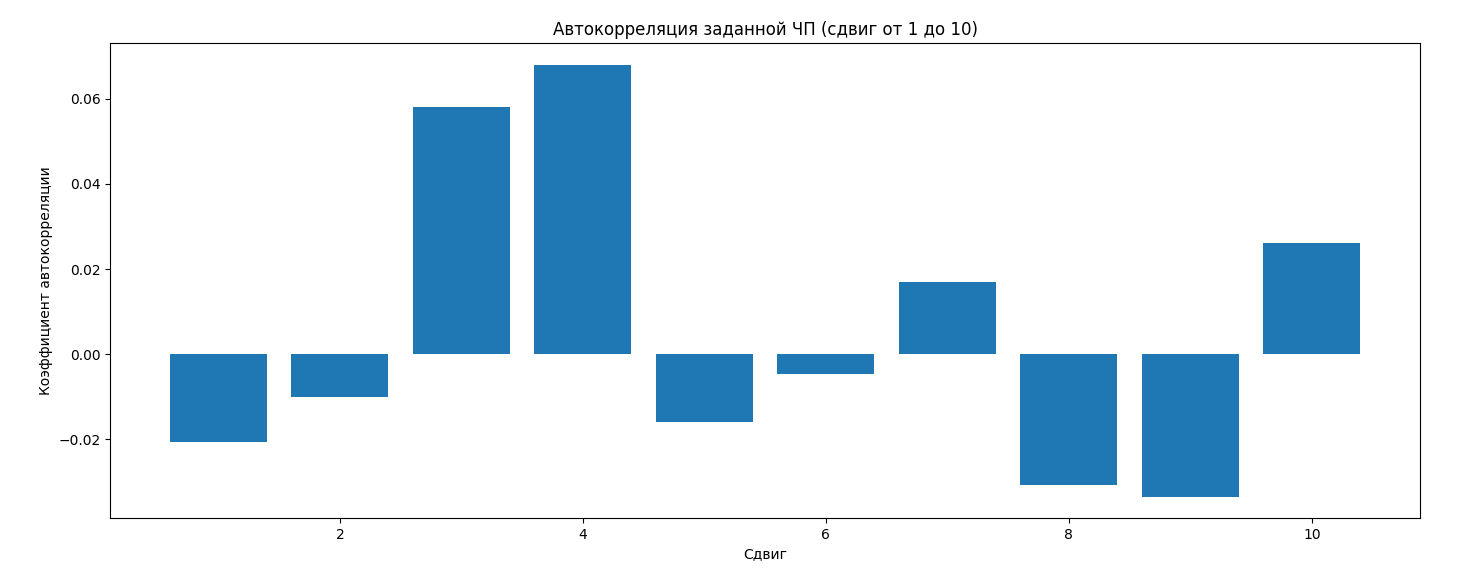
\includegraphics[width=0.8\textwidth]{data/auto_corellation-1.png}
	\caption{Автокорреляционный анализ для заданной последовательности}
\end{figure}

Автокорреляция в сути своей показывает зависимость между текущими данными и предыдущими значениями для выявления
тенденций в последовательностях (т.е. чтобы по предыдущим значениям мы имели возможность предсказать
следующие).

В качестве порогового значения, превышение которого говорит о том, что последовательность неслучайна, нами было выбрано
значение 0.2, и, как мы убедились во время проведения работы, ни для одного из сдвигов коэффициенты автокорреляции не
превышали даже 0.1, из чего мы можем предполагать, что заданная числовая последовательность является случайной.

\begin{figure}[H]
	\centering
	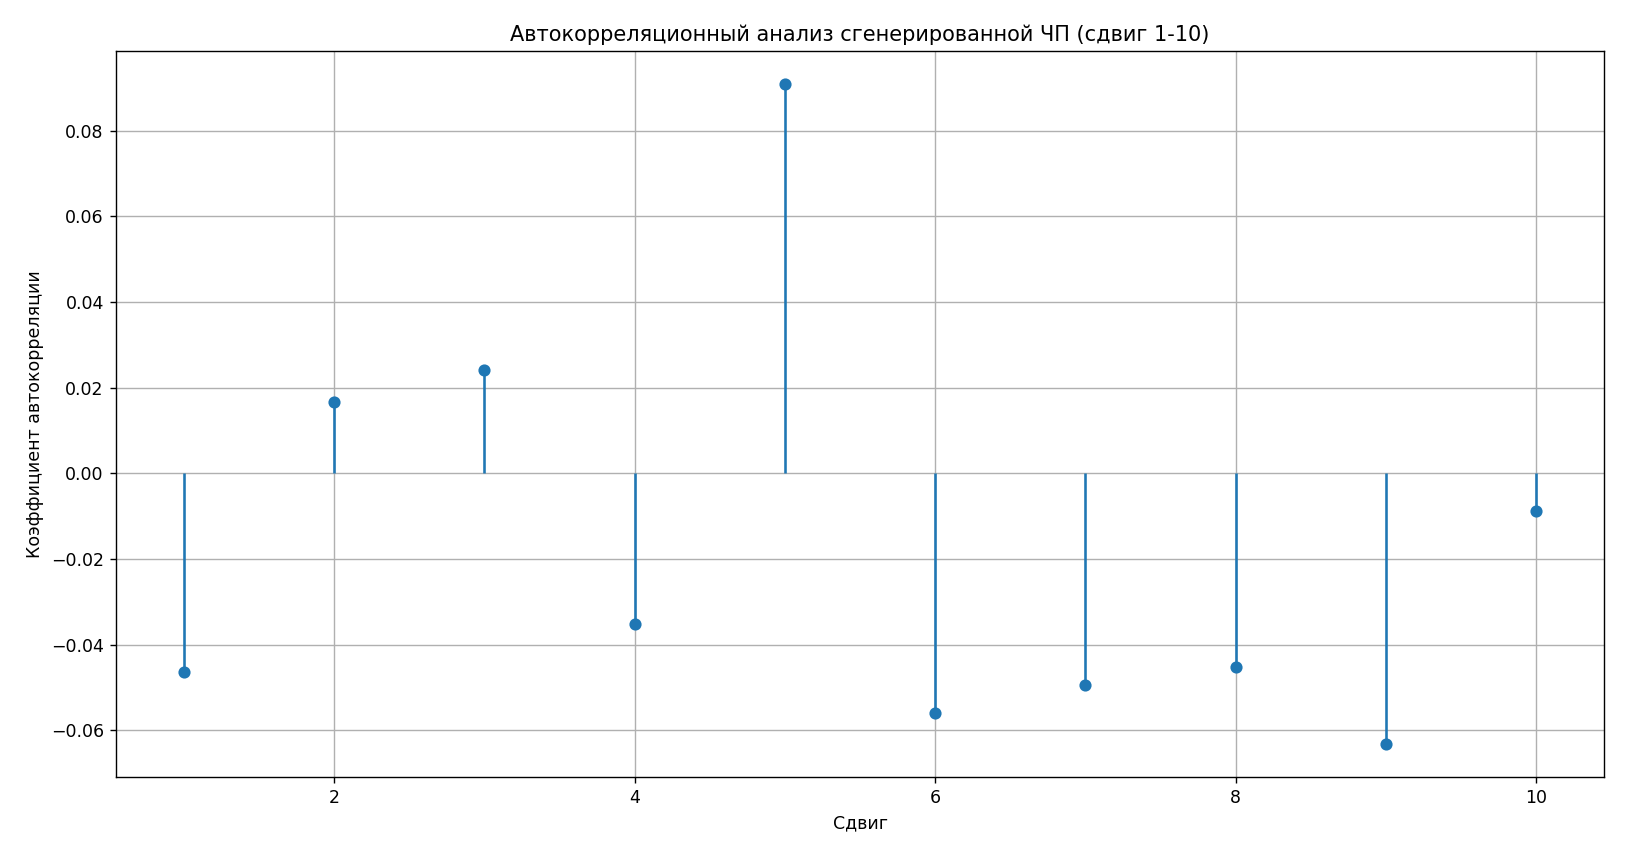
\includegraphics[width=0.75\textwidth]{data/auto_corellation-2.png}
	\caption{Автокорреляционный анализ для сгенерированной последовательности}
\end{figure}

Автокорреляционный анализ сгенерированной числовой последовательности даёт нам аналогичные результаты: ни одно из
значений коэффициентов автокорреляции не превышало 0.1, не говоря уже о 0.2, из чего мы можем делать вывод, что
генерируемая нами последовательность не только случайна, но и приближена к заданной.
